\chapter{設計}
\label{chap:design}

\section{Rive日本語入力システム}

Rive日本語入力システムは以下のものによって構成されている

\begin{itemize}
  \item Rive Client
  \item Rive Server
  \item Rive Analytics
  \item Rive BtachProcessing
  \item Rive Webservice
\end{itemize}

これらのシステムがお互いに作用することで
Rive日本語入力システムが実現されている。

\begin{figure}[htbp]
  \begin{center}
    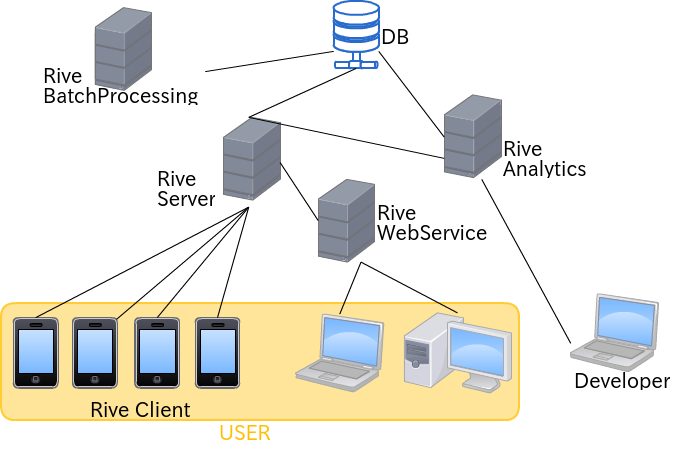
\includegraphics[width=12cm,bb=0 0 540 448]{images/systemstructure.png}
  \end{center}
  \caption{システム全体構成図}
  \label{fig:systemstructure}
\end{figure}


% 各要素について1行ぐらいで軽く説明する
% システム図みたいなので全体を説明する

\section{Rive Client}
\subsection{概要}
モバイルデバイスで利用可能なアプリケーション本体。
\subsection{実装}
AndroidOS\cite{android}向けのIMEとして実装した。


\section{Rive Server}
\subsection{概要}
Rive Clientと通信し、適切な候補単語を推測するシステムの総称。

\subsection{実装}
Node.js\cite{nodejs}を使って実装した。

\section{Rive Analytics}
\subsection{概要}
文字入力のデータを受け取り解析することでシステムの向上に役立てる
\subsection{実装}
Rive Clientからデータを受け取りバージョンごとに管理する

\section{Rive BatchProcessing}
\subsection{概要}
定期的に処理を行うシステムの総称
\subsection{実装}
インターネット上のデータをクロールする

\section{Rive WebService}
\subsection{概要}
システムを試用するためのWEBページとして実装。
また本システムの紹介も兼ねている。
\subsection{実装}
WEBページとして実装した。

\section{システム間通信}
\subsection{実装}
システム間はWebsocketまたはhttpによって実現した。
